\documentclass[dutch]{ltugboat}
\usepackage{babel}
\usepackage[T1]{fontenc}
\usepackage{graphicx}
\usepackage{microtype}
\usepackage[hidelinks,pdfa]{hyperref}
\usepackage{listings}
\usepackage{ulem}
\usepackage{wasysym}
%\title{Documentvariabelen met YAML}
\title{Optimaliseer Documentautomatisering met lua-placeholders in LaTeX}

% repeat info for each author; comment out items that don't apply.
\author{Erik Nijenhuis}
\address{Frans Halsstraat 38\\ Leeuwarden, 8932 JC \\ The Netherlands}
\netaddress{erik (at) xerdi dot com}
\personalURL{https://www.xerdi.com}
%\ORCID{0}
% To receive a physical copy of the TUGboat issue, please include the
% mailing address we should use, as a comment if you prefer it not be printed.

\def\pkg#1{\texttt{#1}\cite{#1}}

\lstset{columns=fullflexible}

\begin{document}
    \maketitle

    \begin{abstract}
        Dit artikel demonstreert hoe documentvariabelen gespecificeerd en aangeleverd kunnen worden in YAML en hoe dat vervolgens kan helpen binnen systeemintegratie aan de hand van een open-source factuur applicatie.
    \end{abstract}

    \section*{Keywords}
    \LuaTeX, \LuaLaTeX, YAML, \sout{Python}

    \section{Inleiding}
    Tijdens een opdracht voor juristen, waarbij de behoefte ontstond om klantinformatie te anonimiseren in overeenkomsten en voorwaarden, ondervond ik de beperkingen van het direct integreren van \LaTeX\ in software, zoals eerder ervaren bij de ontwikkeling van GinVoice\cite{ginvoice}.
    Deze ervaring leidde tot de noodzaak van een betere oplossing om \LaTeX-documenten en data te scheiden.
    Mijn keuze viel op YAML als een geschikte notatie voor het specificeren en aanleveren van data voor LaTeX-documenten.
    Dit vormde de aanleiding voor de ontwikkeling van het LaTeX-pakket \pkg{lua-placeholders}, geschreven met \LuaLaTeX.
    Met dit pakket kunnen juristen een enkele juridische bron hanteren voor meerdere klanten in dezelfde branche, terwijl de klantinformatie wordt geanonimiseerd.
%    In deze inleiding zal ik mijn motivatie, keuzes en implementatie van lua-placeholders nader toelichten.

    \subsection{De Compiler}
    Mijn besluit om LuaLaTeX als compiler te gebruiken, was gebaseerd op verschillende overwegingen en ervaringen.
    Als ervaren ontwikkelaar, met name in het bouwen van Game Engines, had ik uitgebreide ervaring opgedaan met het schrijven van taal koppelingen tussen \Cplusplus\ en Lua voor game-ontwikkeling.
    Deze ervaring stelde me in staat om de kracht van Lua als scripttaal volledig te benutten.

    Een cruciale factor voor mijn keuze was de noodzaak van YAML-support.
    Lua biedt een eenvoudige en effectieve manier om YAML te verwerken, iets wat niet zo naadloos mogelijk is binnen het LaTeX-framework.
    De flexibiliteit en expressiviteit van Lua maakten het mogelijk om YAML-functionaliteit in te bouwen en zo de gewenste scheiding tussen LaTeX-documenten en de bijbehorende data te bewerkstelligen.

    Tijdens mijn onderzoek stuitte ik op de documentatie van het LaTeX-pakket \pkg{markdown}, waar YAML-ondersteuning werd vermeld in combinatie met Jekyll-data.
    Dit was een aanvullende bevestiging dat LuaLaTeX de meest geschikte compiler was voor mijn specifieke behoeften.

    \subsection{Wat is YAML?}
    YAML, wat oorspronkelijk stond voor ``Yet Another Markup Language'' of speels gezegd ``YAML Ain't Markup Language'', is een op mensentaal gebaseerde opmaaktaal voor het serialiseren van gegevens.
    In plaats van zich te richten op markeringen zoals bij traditionele opmaaktalen, legt YAML de nadruk op leesbaarheid en eenvoud.
    Het wordt veel gebruikt in verschillende toepassingen vanwege zijn menselijke leesbaarheid en flexibiliteit.

    YAML vindt diverse toepassingen, waaronder configuratiebestanden voor tools zoals Docker Compose, Jekyll-sites, Kubernetes-configuraties en Travis CI. Deze veelzijdigheid maakt het een populaire keuze voor het specificeren van gegevensstructuren op een begrijpelijke manier.
    In de context van dit artikel is YAML cruciaal voor het flexibel specificeren van documentvariabelen en biedt het een gestructureerde manier om gegevens aan te leveren voor het genereren van LaTeX-documenten met \pkg{lua-placeholders}.


    \section{Legacy Factuur}
    Om een goed voorbeeld te geven van de features en toegevoegde waarde van \pkg{lua-placeholders} pakken we de \LaTeX-code van GinVoice\footnote{Volledige broncode: \url{https://gitlab.gnome.org/MacLotsen/ginvoice/-/tree/master/res/basic_template}}.
    Daarnaast houd ik rekening met de volgende doelen:
    \begin{enumerate}
        \item De factuurtemplate dient gecompileerd te worden, ook wanneer er geen waardes beschikbaar zijn.
        \item Alle factuurtemplates gebruiken dezelfde YAML-specificatie, zodat het verschillende templates, bijvoorbeeld met de \texttt{scrlttr2} klasse, gekoppeld kunnen worden aan de applicatie.
        \item De variabele kolomdefinitie laten we achterwege, aangezien dit het aanzienlijk lastiger maakt voor \LaTeX\ gebruikers die iets anders dan de \texttt{longtable} willen gebruiken.
        \item De factuurtemplate kan ook zonder applicatie werken, speciaal voor de \LaTeX-minimalisten onder ons.
    \end{enumerate}

    \subsection{\LaTeX-template}
    Belangrijk om te weten van de huidige implementatie is dat GinVoice\cite{ginvoice} een Python script -- \texttt{generator.py} -- gebruikt om extra \TeX-bestanden te genereren.
    Die \TeX-bestanden worden vervolgens in de template ingeladen, zodat de benodigde macro's beschikbaar zijn.
    Uiteraard zal dat niet meer het geval zijn na het introduceren van \pkg{lua-placeholders}.
    Hier is de code binnen de \texttt{document} omgeving:
    \lstinputlisting[name=invoice-original,language={[LaTeX]TeX},firstnumber=52,linerange={52-55},numbers=left,xleftmargin=15pt]{invoice-original.tex}
    De eerste drie regels hebben enkel te maken met de \cs{makeheader} macro afkomstig van \texttt{invoice.cls} en in de preamble van dit bestand is er een gekleurde laag aan toegevoegd met behulp van een pakket uit KommaScript—\pkg{scrlayer-scrpage}.
    \lstinputlisting[name=invoice-original,language={[LaTeX]TeX},firstnumber=56,linerange={56-67},numbers=left,xleftmargin=15pt]{invoice-original.tex}
    Deze bijzondere \texttt{tabular} constructie zorgt ervoor dat de klantinformatie links komt te staan en de leveranciersinformatie rechts.
    Niet echt een waardig voorbeeld als je het vergelijkt met bijvoorbeeld de \pkg{scrlttr2} klasse, echter hoort het gegeven voorbeeld de standaard factuur template binnen de applicatie te zijn.
    Iets wat ik helaas nog niet heb kunnen realiseren binnen GinVoice\cite{ginvoice}.
    \lstinputlisting[name=invoice-original,language={[LaTeX]TeX},firstnumber=69,linerange={69-72},numbers=left,xleftmargin=15pt]{invoice-original.tex}
    Op regel 69 zie je dat het gegenereerde \TeX-bestand verlaat wordt ingeladen.
    Dit heeft typisch te maken met het calculatieproces van de kolombreedtes.
    Namelijk, de pagina dimensies zijn in de preamble nog onbekend, of kunnen nog veranderen.
    Een opmerkelijke functionaliteit daarentegen is de variabele kolomdefinitie, iets wat met \pkg{lua-placeholders} alsnog knap lastig kan worden.
    \lstinputlisting[name=invoice-original,language={[LaTeX]TeX},firstnumber=74,linerange={74-78},numbers=left,xleftmargin=15pt]{invoice-original.tex}
    Tot slot, een bericht waarin bijvoorbeeld bedragen en betaaltermijnen in gespecificeerd kunnen worden met daaronder optioneel drie plaatjes voor bijvoorbeeld logo's van partners of andere betrokken instanties van de bedrijfsvoering.
    \lstinputlisting[name=invoice-original,language={[LaTeX]TeX},firstnumber=80,linerange={80-81},numbers=left,xleftmargin=15pt]{invoice-original.tex}
    \subsection{Factuur Data}\label{sub:invoice data}
    Grof gezegd komt de data van de factuur op het volgende neer:
    \begin{itemize}
        \item Factuurinformatie
        \item Klantinformatie
        \item Leveranciersinformatie
        \item Factuurregels
        \item Slottekst
    \end{itemize}
    Met enige details daar gelaten.

    \subsection{Resultaat Voorbeeld}
    Het project zelf heeft voorbeelddata wat het volgende voorbeeld geeft:\\
    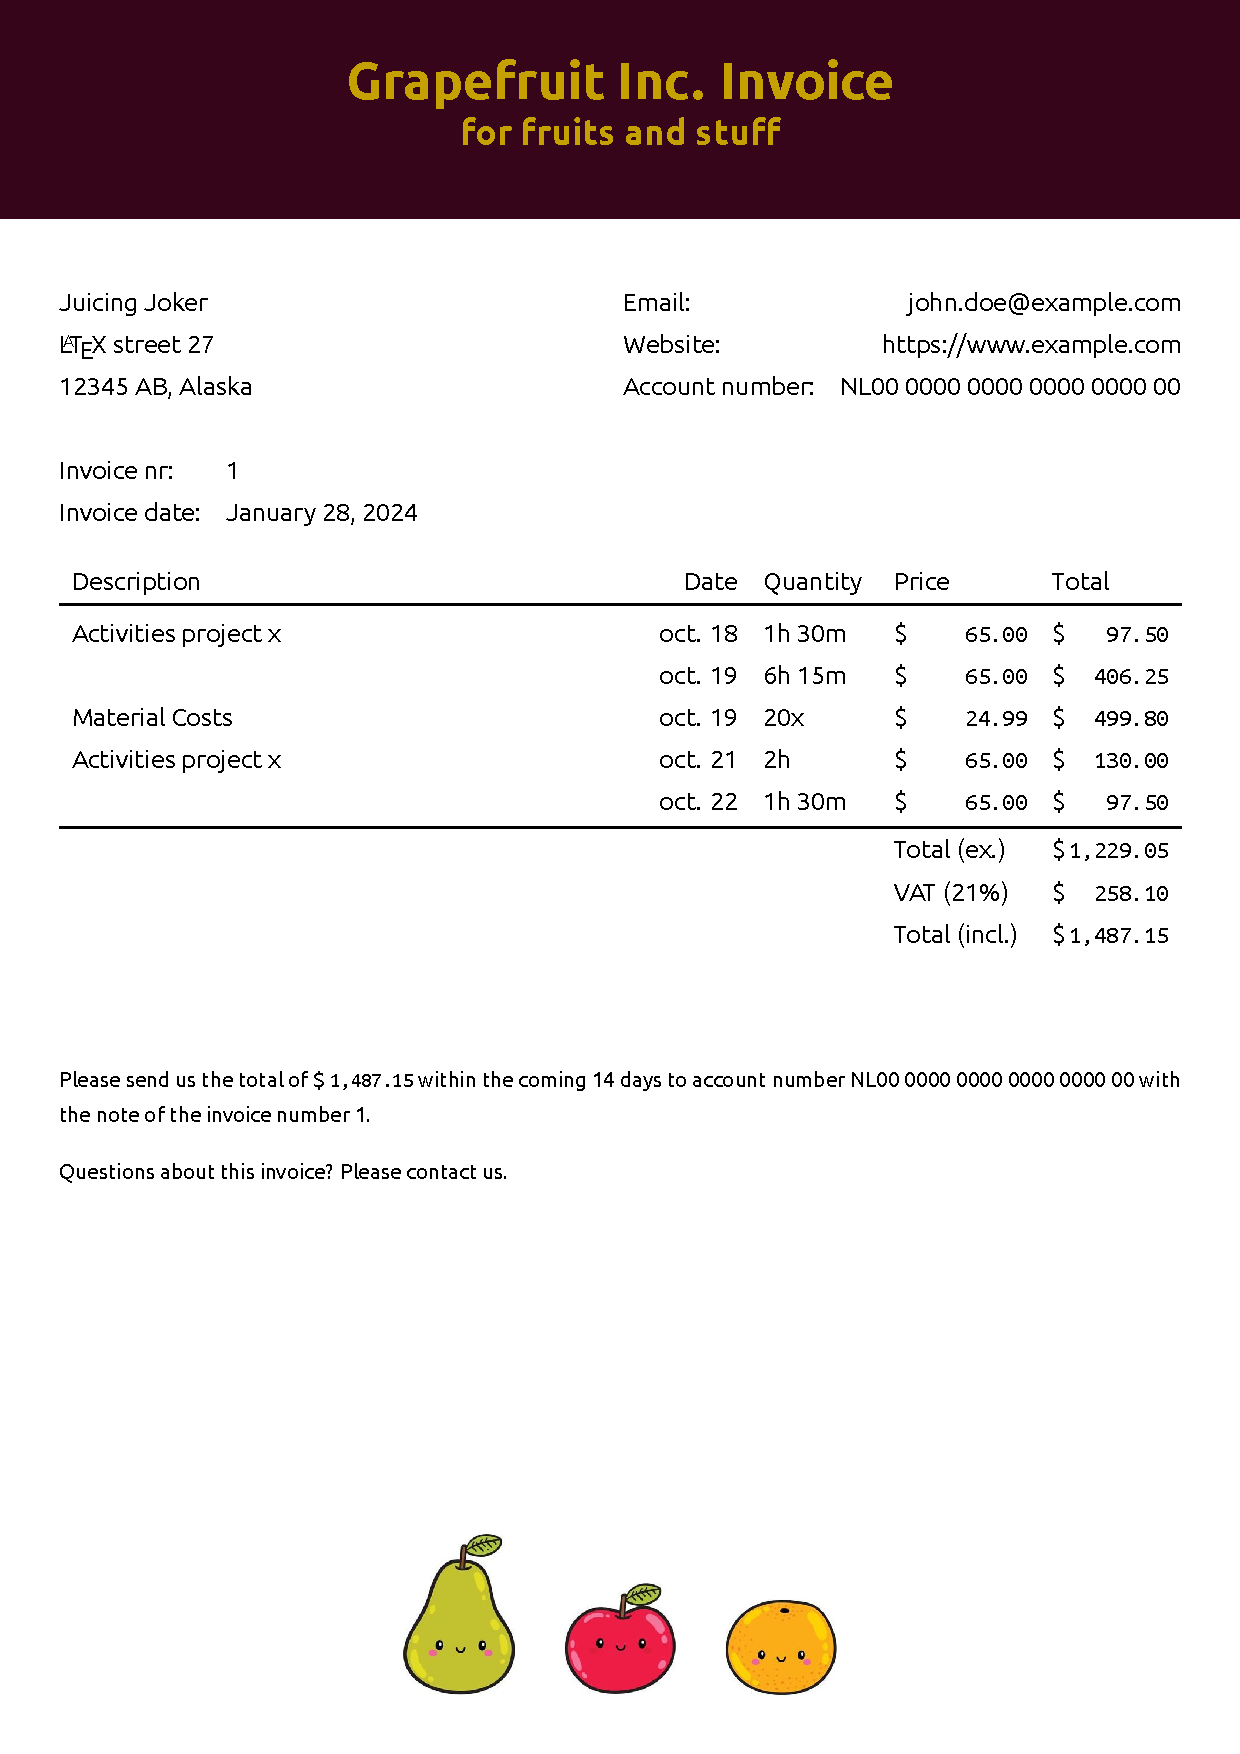
\includegraphics[width=\linewidth]{ginvoice.pdf}
    % Bespreking van de voordelen van het gebruik van lua-placeholders voor documentautomatisering.
    Echter, zoals het nu is, zou je Python nodig hebben om dit voorbeeld te kunnen maken.
    Ervan uit gaande dat template makers voornamelijk \LaTeX\ beheersen, is dat voor deze gebruikers onwenselijk.
    Daar gaan we nu verandering in brengen, maar dan uitsluitend met \LuaLaTeX.

    \section{YAML-Interfaces met \texttt{lua-placeholders}}
    Kijkend naar de benodigde data in hoofdstuk~\ref{sub:invoice data} zien we verschillende data types voorbij komen.
    Hoewel, de meeste data simpelweg van het type \texttt{string} is, zoals de titel, subtitel en slottekst, zijn er ook nog de zeer uitdagende structuren, zoals voor de factuurregels, klant- en leveranciersinformatie.

    % Concrete voorbeelden van hoe lua-placeholders zijn toegepast in echte situaties.
    Hier is een mogelijke YAML-specificatie voor de factuur met voor nu placeholders daar gelaten:
    \lstinputlisting[language=YAML,numbers=left,xleftmargin=15pt]{yaml-spec.yaml}
    Als we dit voorbeeld zouden inladen met:\\\lstinline[language={[LaTeX]TeX}]|\loadrecipe[\jobname]{invoice-recipe.yaml}|,\\dan zouden we ontzettend veel te maken krijgen met de \cs{paramfield} macro of de \texttt{paramobject} omgeving, dankzij de veelvoudige keuze voor het type \texttt{object}.
    De reden voor \cs{jobname} is zodat de waarden onder de \textit{standaard} namespace komen te staan, wat iedere aanhaling net iets vereenvoudigd door het niet hoeven opgeven van een optionele \meta{namespace}.

    \subsection{Header (Object)}
    Wat eerder neer kwam op \cs{makeheader}, gaat helaas nu niet meer op.
    Een bijzonder hinderlijke keuze was het, om het gegenereerde bestand \texttt{meta.tex} vanuit \texttt{invoice.cls} in te laden.
    Voor de nieuwe versie is dit ongewenst, en ik raad het je ook zeker \underline{niet} aan om data in documentklassen te verwerken.

    Voor nu gaan we er van uit dat \texttt{invoice.cls} zodanig is aangepast dat het geen fouten meer veroorzaakt en vergeten we het bestaan van \cs{makeheader} en vervangen we dat met:
    \lstinputlisting[name=invoice-evidence,language={[LaTeX]TeX},linerange={48-55},gobble=4]{invoice-evidence.tex}
    In het voorbeeld zijn er maar twee verschillen met betrekking tot de nieuwe versie, namelijk:\\
    \cs{title} \textrightarrow \lstinline[language={[LaTeX]TeX}]|\paramfield{header}{title}|\\
    \cs{subtitle} \textrightarrow \lstinline[language={[LaTeX]TeX}]|\paramfield{header}{subtitle}|

    Echter, kunnen \cs{title} en \cs{subtitle} alsnog beschikbaar gemaakt worden door het gebruik van de \texttt{paramobject} omgeving:
    \begin{lstlisting}[language={[LaTeX]TeX}]
\begin{paramobject}{header}
    \begin{center}
        \color{textcolor}
        {\Huge\textbf{\title}\\}
        \vspace{-.3cm}
        {\Large\textbf{\subtitle}\\}
    \end{center}
\end{paramobject}
    \end{lstlisting}
    De keuze voor een \texttt{object} ten opzichte van de titel en subtitel als directe \texttt{string}s in de specificatie heeft in dit geval te maken met de bestaande interface op applicatie niveau.
    Het gebruik van het \texttt{object} heeft geen meerwaarde voor nieuwe situaties en als het korter kan, ga dan voor korter.

    % Mogelijkheden voor systeemintegratie en automatisering met lua-placeholders.
    % Vergelijking met alternatieve methoden en waarom lua-placeholders de beste keuze waren.

    \subsection{Informatie}

    \subsection{Tabel}

    \subsection{Slottekst}

    \section{Uitvoering}
    % Geavanceerde YAML payload voorbeelden
    \subsection{De Template Versie}
    \setlength\fboxsep{0pt}
    \fbox{\includegraphics[width=\linewidth]{invoice-evidence-tmpl.pdf}}

    \subsection{Ingevulde Versie}
    % Overwegingen voor anderen die overwegen dit pakket te gebruiken.

    % notes on ginvoice
    % Removed the \global\def\currency{\$}
\global\def\author{Erik Nijenhuis}
\global\def\title{Grapefruit Inc. Invoice}
\global\def\subject{Invoice for Juicing Joker}
\global\def\keywords{Invoice Grapefruit Juicing Joker}
\global\def\producer{GinVoice Generator}
\global\def\creator{gingen}
\global\def\continuationheader{\title{} -- \subject{}}
\global\def\continuationfooter{See next page.}
 from invoice.cls
    % Removed the hypersetup

    \section{Interfaces Opsplitsen}
    % Intro met Git structuur
    % Reintroduceer missende dingen met een aparte style.yaml

    % Opsplitsen in bedrijfs template, klant template, daadwerkelijke factuur met Git

    \section{Conclusie}
    % Samenvatting van hoe lua-placeholders hebben bijgedragen aan het optimaliseren van documentautomatisering.
    % Aansporing voor lezers om lua-placeholders te verkennen en te implementeren in hun eigen projecten.

    \bibliographystyle{tugboat}%
    \nocite{book-minimal}      % make the example bibliography non-empty
    \bibliography{erik}       % xampl.bib comes with BibTeX

    \makesignature
\end{document}
